\section{Proces uczenia}
\label{sec:training-process}

Z racji, że stworzono zestaw danych, który umożliwiał pełną kontrolę nad etykietowaniem danych, każda sekwencja w zestawie była poprawna. Dodatkowo nagrania były na bieżąco weryfikowane jednorazowym odtworzeniem.

\begin{table}[H]
    \centering
    \small
    \begin{tabular}[c]{|l|r|}
        \hline
        Czas trwania             & 00:00:02 \\ \hline
        Prędkość obrazu          & 30 FPS   \\ \hline
        Przeciętny rozmiar pliku & 393 KB   \\ \hline
        Szerokość klatki         & 1280     \\ \hline
        Wysokość klatki          & 720      \\ \hline
    \end{tabular}
    \caption{Specyfikacja filmu}
    \label{tab:film-specs}
\end{table}

Po dokonaniu ekstrakcji koordynatów z nagrań, nie zaobserwowano pustych wartości. Dzięki korzystnym warunkom oświetlenia podczas nagrań, wszystkie 36000 plików zawierało po 30 wierszy. Oznacza to, model detekcji MediaPipe rozpoznał w każdej klatce wszystkich filmów co najmniej jedną rękę z co najmniej 50\% pewnością. Konwersja na mniejszą prędkość klatek filmu nie pogorszyła jakości plików. Filmy tych samych wymiarów o prędkości 15 FPS ważyły średnio 151 KB, natomiast pliki CSV już 40 KB. W rezultacie, do przetworzenia było dużo mniej danych.

Danymi wejściowymi każdej klasyfikacji była lista 30 konkretnych sekwencji 63 parametrów położenia zamiast 30 kadrów filmu. Była to spłaszczona struktura listy o jeden wymiar. Wiersz tabeli zawierał wszystkie 21 koordynatów relatywnego położenia od nadgarstka. Współrzędne każdego punktu występowały po sobie w takiej samej kolejności jak zwracał je MediaPipe z każdej detekcji.

\begin{figure}[H]
    \centering
    \includesvg[width=0.4\linewidth]{figures/hand}
    \caption{Punkty dłoni}
    \label{fig:hand-landmarks-mp}
\end{figure}

\begin{table}[H]
    \centering
    \small
    \begin{tabular}[c]{|r|l|}
        \hline
        \thead{Indeks} & \thead{Nazwa anatomiczna}                        \\ \hline
        0              & Nadgarstek                                       \\ \hline
        1              & Staw nadgarstkowo-śródręczny kciuka              \\ \hline
        2              & Staw śródręczno-paliczkowy kciuka                \\ \hline
        3              & Staw międzypaliczkowy kciuka                     \\ \hline
        4              & Paliczek dalszy kciuka                           \\ \hline
        5              & Staw śródręczno-paliczkowy palca wskazującego    \\ \hline
        6              & Staw międzypaliczkowy bliższy palca wskazującego \\ \hline
        7              & Staw międzypaliczkowy dalszy palca wskazującego  \\ \hline
        8              & Paliczek dalszy palca wskazującego               \\ \hline
        9              & Staw śródręczno-paliczkowy palca środkowego      \\ \hline
        10             & Staw międzypaliczkowy bliższy palca środkowego   \\ \hline
        11             & Staw międzypaliczkowy dalszy palca środkowego    \\ \hline
        12             & Paliczek dalszy palca środkowego                 \\ \hline
        13             & Staw śródręczno-paliczkowy palca serdecznego     \\ \hline
        14             & Staw międzypaliczkowy bliższy palca serdecznego  \\ \hline
        15             & Staw międzypaliczkowy dalszy palca serdecznego   \\ \hline
        16             & Paliczek dalszy palca serdecznego                \\ \hline
        17             & Staw śródręczno-paliczkowy palca małego          \\ \hline
        18             & Staw międzypaliczkowy bliższy palca małego       \\ \hline
        19             & Staw międzypaliczkowy dalszy palca małego        \\ \hline
        20             & Paliczek dalszy palca małego                     \\ \hline
    \end{tabular}
    \caption{Kolejność indeksów MediaPipe dla stawów i kości ręki}
    \label{tab:mediapipe-keypoint-indices}
\end{table}

Struktura warstw pierwszego modelu była bardzo prosta. Między warstwami wejścia i wyjścia znajdowała się jedynie warstwa LSTM. Wytrenowano model klasyfikacji na mniejszej liczbie epok, aby uniknąć przetrenowania~\cite{dietterich1995}.

\begin{figure}[H]
    \centering
    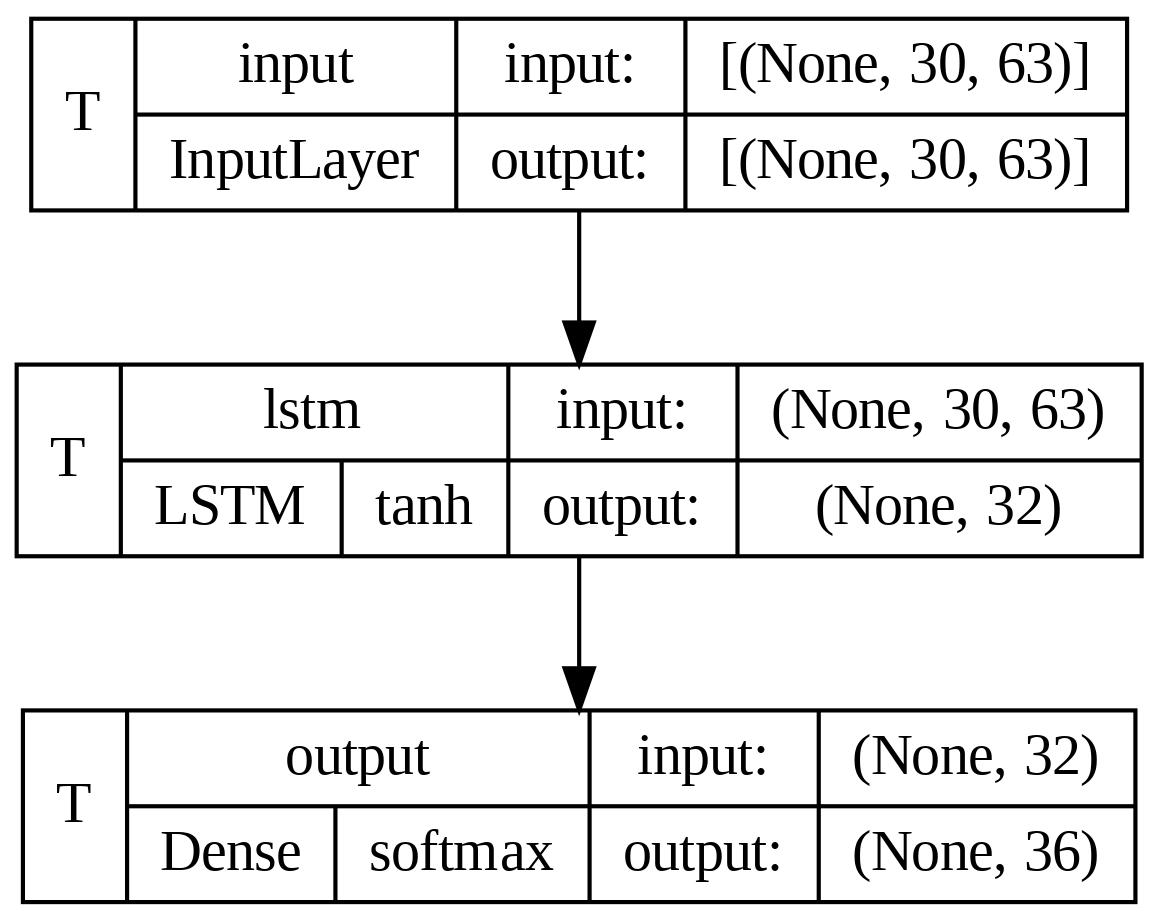
\includegraphics[width=0.5\textwidth]{figures/initial-layers}
    \caption{Architektura warstw pierwszego modelu}
    \label{fig:initial-layers}
\end{figure}

Wartość funkcji straty pierwszego modelu wynosiła $0.0966$, a jego średnia dokładność klasyfikacji $0.9732$. Mimo wysokiego wyniku, wciąż zaobserwowano liczne fałszywe rezultaty. Wyniki pierwszego modelu wyglądały obiecująco, ale było miejsce na poprawę.

\begin{figure}[H]
    \centering
    \begin{subfigure}[H]{0.49\textwidth}
        \centering
        \begin{tikzpicture}
            \begin{axis}[legend pos=north east]
                \addplot[color=train]
                coordinates {
                        (0, 2.4204294681549072)
                        (1, 1.2742657661437988)
                        (2, 0.8588921427726746)
                        (3, 0.5741569399833679)
                        (4, 0.47340530157089233)
                        (5, 0.5858796238899231)
                        (6, 0.3992736339569092)
                        (7, 0.3969440460205078)
                        (8, 0.334946870803833)
                        (9, 0.2724245488643646)
                        (10, 0.2528952658176422)
                        (11, 0.31386426091194153)
                        (12, 0.2887764573097229)
                        (13, 0.33818042278289795)
                        (14, 0.24940292537212372)
                        (15, 0.1675003618001938)
                        (16, 0.13600265979766846)
                        (17, 0.17713148891925812)
                        (18, 0.15159308910369873)
                        (19, 0.11480425298213959)
                        (20, 0.1541949212551117)
                        (21, 0.10616244375705719)
                        (22, 0.09303811192512512)
                        (23, 0.07700393348932266)
                        (24, 0.10956569761037827)
                    };
                \addplot[color=validation]
                coordinates {
                        (0, 1.598986268043518)
                        (1, 1.0582579374313354)
                        (2, 0.6733798384666443)
                        (3, 0.5364265441894531)
                        (4, 0.4366495907306671)
                        (5, 0.6216613054275513)
                        (6, 0.30982089042663574)
                        (7, 0.37502381205558777)
                        (8, 0.2651835083961487)
                        (9, 0.2687380611896515)
                        (10, 0.24191896617412567)
                        (11, 0.2596803307533264)
                        (12, 0.962278425693512)
                        (13, 0.28931111097335815)
                        (14, 0.19661971926689148)
                        (15, 0.17439985275268555)
                        (16, 0.13117994368076324)
                        (17, 0.16091205179691315)
                        (18, 0.16446831822395325)
                        (19, 0.11679905652999878)
                        (20, 0.12194940447807312)
                        (21, 0.1308525651693344)
                        (22, 0.07499074935913086)
                        (23, 0.07690116763114929)
                        (24, 0.10444225370883942)
                    };
                \legend{loss, val\_loss}
            \end{axis}
        \end{tikzpicture}
        \caption{Straty pierwszego modelu}
        \label{fig:initial-loss}
    \end{subfigure}
    \hfill
    \begin{subfigure}[H]{0.49\textwidth}
        \centering
        \begin{tikzpicture}
            \begin{axis}[legend pos=south east]
                \addplot[color=train]
                coordinates {
                        (0, 0.2479938268661499)
                        (1, 0.5650848746299744)
                        (2, 0.719367265701294)
                        (3, 0.8231095671653748)
                        (4, 0.8528163433074951)
                        (5, 0.8206404447555542)
                        (6, 0.876311719417572)
                        (7, 0.8761188387870789)
                        (8, 0.8954089283943176)
                        (9, 0.9077546000480652)
                        (10, 0.9219521880149841)
                        (11, 0.9050154089927673)
                        (12, 0.8970293402671814)
                        (13, 0.8824459910392761)
                        (14, 0.9195987582206726)
                        (15, 0.9527778029441833)
                        (16, 0.9600694179534912)
                        (17, 0.9456018805503845)
                        (18, 0.957561731338501)
                        (19, 0.9670910239219666)
                        (20, 0.9525848627090454)
                        (21, 0.9668981432914734)
                        (22, 0.970370352268219)
                        (23, 0.9771990776062012)
                        (24, 0.967438280582428)
                    };
                \addplot[color=validation]
                coordinates {
                        (0, 0.4798611104488373)
                        (1, 0.6305555701255798)
                        (2, 0.7840277552604675)
                        (3, 0.8298611044883728)
                        (4, 0.8645833134651184)
                        (5, 0.8031250238418579)
                        (6, 0.9177083373069763)
                        (7, 0.8770833611488342)
                        (8, 0.921875)
                        (9, 0.9229166507720947)
                        (10, 0.934374988079071)
                        (11, 0.9118055701255798)
                        (12, 0.7006944417953491)
                        (13, 0.8954861164093018)
                        (14, 0.953125)
                        (15, 0.9472222328186035)
                        (16, 0.9645833373069763)
                        (17, 0.9524305462837219)
                        (18, 0.9545139074325562)
                        (19, 0.9624999761581421)
                        (20, 0.9635416865348816)
                        (21, 0.9607638716697693)
                        (22, 0.9767361283302307)
                        (23, 0.9760416746139526)
                        (24, 0.9697916507720947)
                    };
                \legend{acc, val\_acc}
            \end{axis}
        \end{tikzpicture}
        \caption{Precyzje pierwszego modelu}
        \label{fig:initial-accuracy}
    \end{subfigure}
    \caption{Krzywe uczenia pierwszego modelu}
    \label{fig:initial-loss-accuracy}
\end{figure}

Tym razem przed szukaniem nowych parametrów modelu zmieniono nieco strukturę warstw w celu zoptymalizowania wyniku. Dodano dodatkowo warstwę porzucenia (ang. dropout layer) oraz warstwę normalizującą próbki danych (ang. batch normalization layer). Targetem była jak najniższa wartość funkcji straty względem zbioru walidacyjnego w celu jak najlepszego rozróżnienia dynamicznych znaków daktylografii.

Abstrahując od później zmienionych parametrów konfiguracji warstwy LSTM i stałej uczenia, warstwa wejściowa oraz wyjściowa się niczym nie różniły w obydwu modelach.

\begin{figure}[H]
    \centering
    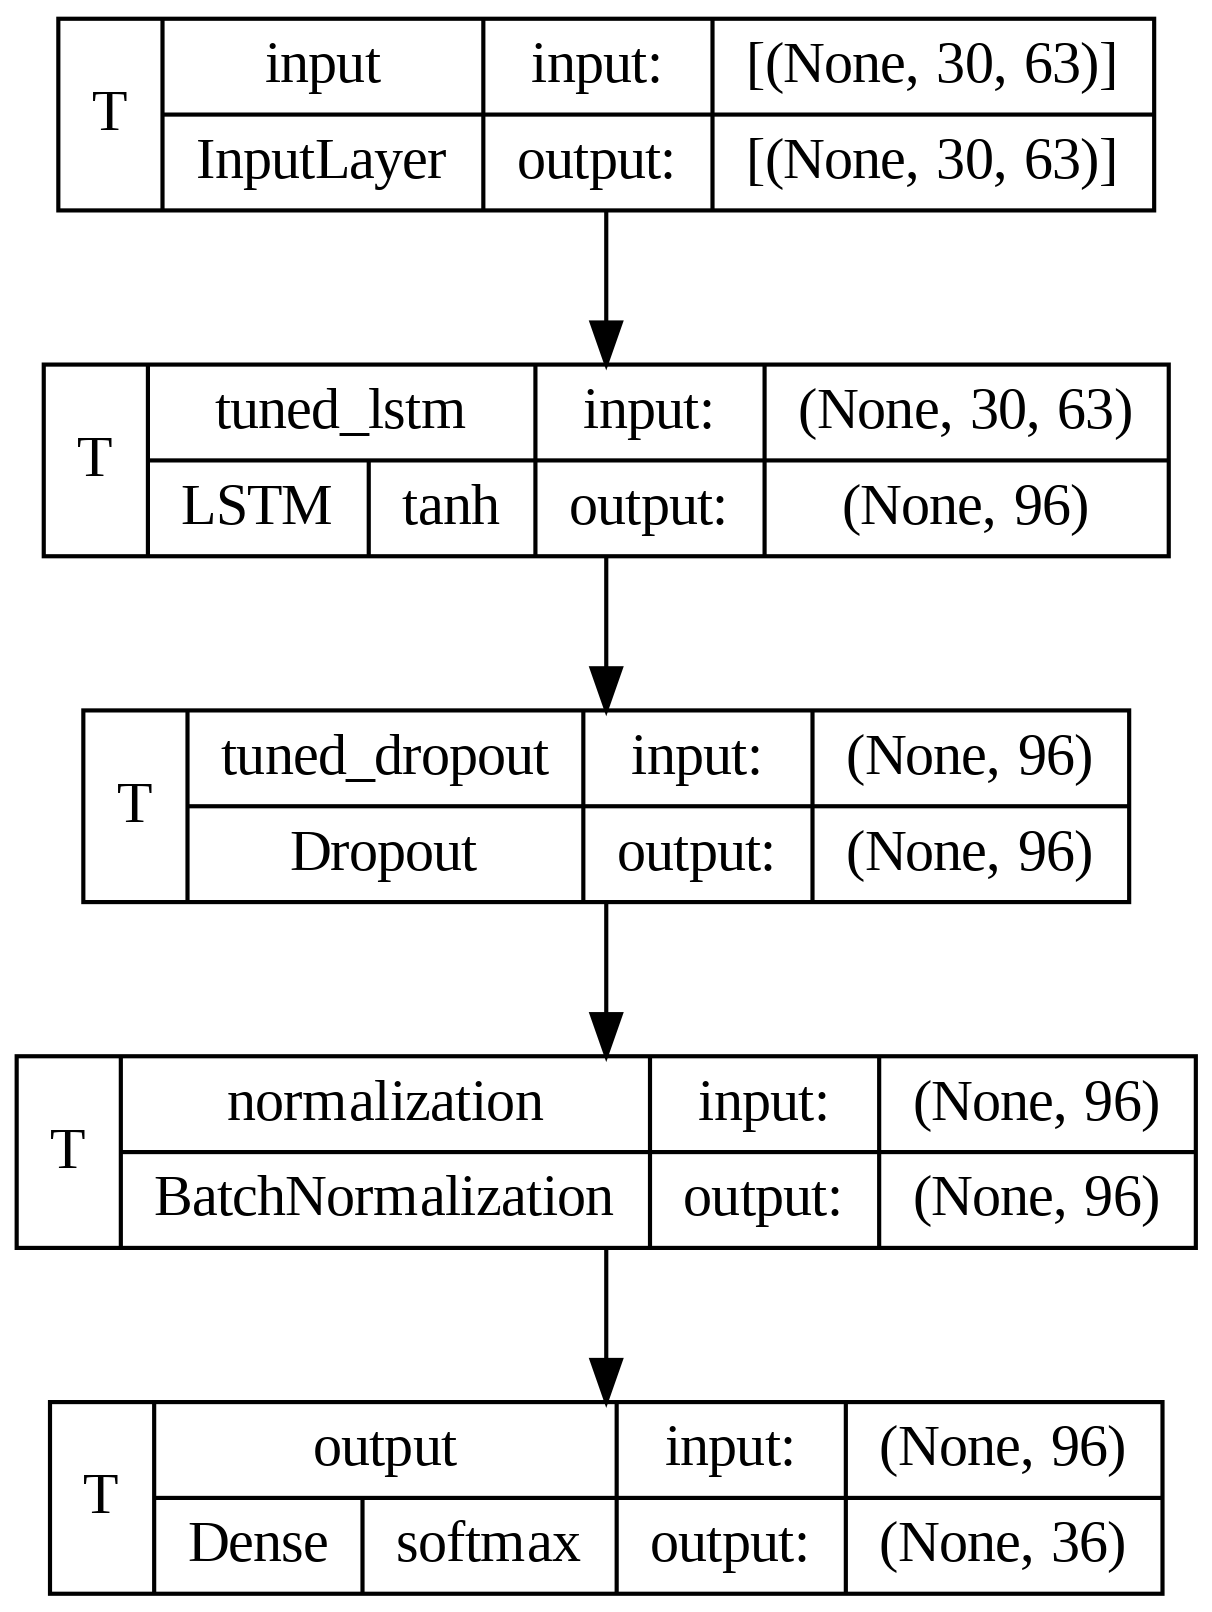
\includegraphics[width=0.5\textwidth]{figures/hypermodel-layers}
    \caption{Architektura warstw hipermodelu}
    \label{fig:hypermodel-layers}
\end{figure}

W rezultacie otrzymano listę optymalnych parametrów modeli, które osiągnęły najniższą wartość funkcji straty. Algorytm porzucał proces uczenia, gdy nie zarejestrował spadku przez 5 epok i przechodził do uczenia na innych parametrach. Niżej zaprezentowana tabela przedstawia 10 najlepszych sesji, gdzie przypadkowo stała uczenia wynosiła $0.001$.

\begin{table}[H]
    \centering
    \small
    \begin{tabular}[c]{|r|r|r|r|r|r|}
        \hline
        \thead{trial} & \thead{val\_loss} & \thead{lstm\_units} & \thead{dropout\_rate} & \thead{epochs} & \thead{initial\_epoch} \\ \hline
        88            & 0.00668           & 96                  & 0.4                   & 50             & 0                      \\ \hline
        72            & 0.00687           & 256                 & 0.2                   & 50             & 17                     \\ \hline
        50            & 0.00908           & 128                 & 0.5                   & 50             & 17                     \\ \hline
        82            & 0.00922           & 160                 & 0.3                   & 50             & 17                     \\ \hline
        89            & 0.01062           & 224                 & 0.5                   & 50             & 0                      \\ \hline
        51            & 0.01070           & 128                 & 0.2                   & 50             & 17                     \\ \hline
        49            & 0.01437           & 128                 & 0.5                   & 17             & 6                      \\ \hline
        48            & 0.01504           & 128                 & 0.2                   & 17             & 6                      \\ \hline
        68            & 0.01648           & 256                 & 0.2                   & 17             & 6                      \\ \hline
        74            & 0.01656           & 160                 & 0.3                   & 17             & 0                      \\ \hline
    \end{tabular}
    \caption{Wyniki szukania hiperparametrów}
    \label{tab:hyperparameters-searches}
\end{table}

Najniższą wartość funkcji straty nowy model osiągnął w 39 epoce. W późniejszych etapach uczenia nie zaobserwowano spadku poniżej $0.0063$.

\begin{figure}[H]
    \centering
    \begin{subfigure}[H]{0.49\textwidth}
        \centering
        \begin{tikzpicture}
            \begin{axis}[legend pos=north east]
                \addplot[color=train]
                coordinates {
                        (0, 0.7400228381156921)
                        (1, 0.16438643634319305)
                        (2, 0.10472238063812256)
                        (3, 0.08075176924467087)
                        (4, 0.06782187521457672)
                        (5, 0.053191252052783966)
                        (6, 0.04474253207445145)
                        (7, 0.04544195905327797)
                        (8, 0.037467993795871735)
                        (9, 0.03376125171780586)
                        (10, 0.03394489735364914)
                        (11, 0.02983199432492256)
                        (12, 0.030097978189587593)
                        (13, 0.02727559022605419)
                        (14, 0.030781995505094528)
                        (15, 0.027794888243079185)
                        (16, 0.026910267770290375)
                        (17, 0.027429260313510895)
                        (18, 0.018912121653556824)
                        (19, 0.023394674062728882)
                        (20, 0.022798802703619003)
                        (21, 0.02527042292058468)
                        (22, 0.019330458715558052)
                        (23, 0.016061274334788322)
                        (24, 0.01659027859568596)
                        (25, 0.020914537832140923)
                        (26, 0.01878662407398224)
                        (27, 0.015272611752152443)
                        (28, 0.012623035348951817)
                        (29, 0.01786784641444683)
                        (30, 0.016267498955130577)
                        (31, 0.014223909005522728)
                        (32, 0.013478400185704231)
                        (33, 0.020879050716757774)
                        (34, 0.010418623685836792)
                        (35, 0.012312478385865688)
                        (36, 0.014746789820492268)
                        (37, 0.015016404911875725)
                        (38, 0.010981113649904728)
                        (39, 0.012060846202075481)
                        (40, 0.013025358319282532)
                        (41, 0.012648425064980984)
                        (42, 0.012041987851262093)
                        (43, 0.013749206438660622)
                        (44, 0.012377619743347168)
                        (45, 0.010463446378707886)
                        (46, 0.010169493965804577)
                        (47, 0.011186471208930016)
                        (48, 0.012575146742165089)
                        (49, 0.006315256003290415)
                    };
                \addplot[color=validation]
                coordinates {
                        (0, 0.2216375768184662)
                        (1, 0.10178261995315552)
                        (2, 0.06807278096675873)
                        (3, 0.1186809241771698)
                        (4, 0.11059701442718506)
                        (5, 0.03363170474767685)
                        (6, 0.024100832641124725)
                        (7, 0.07771452516317368)
                        (8, 0.03408350795507431)
                        (9, 0.05639881640672684)
                        (10, 0.031560614705085754)
                        (11, 0.03259143978357315)
                        (12, 0.026484370231628418)
                        (13, 0.023458261042833328)
                        (14, 0.03281714767217636)
                        (15, 0.02685055509209633)
                        (16, 0.0253053717315197)
                        (17, 0.033115506172180176)
                        (18, 0.01989421434700489)
                        (19, 0.024947768077254295)
                        (20, 0.027721939608454704)
                        (21, 0.02230708673596382)
                        (22, 0.01142285019159317)
                        (23, 0.013582443818449974)
                        (24, 0.011441645212471485)
                        (25, 0.01860242523252964)
                        (26, 0.012406373396515846)
                        (27, 0.013386434875428677)
                        (28, 0.0250511784106493)
                        (29, 0.01650191657245159)
                        (30, 0.013023875653743744)
                        (31, 0.018163375556468964)
                        (32, 0.018555518239736557)
                        (33, 0.014497698284685612)
                        (34, 0.012299811467528343)
                        (35, 0.01222353894263506)
                        (36, 0.00880603026598692)
                        (37, 0.01093954499810934)
                        (38, 0.006311490666121244)
                        (39, 0.031178146600723267)
                        (40, 0.016455428674817085)
                        (41, 0.008012923412024975)
                        (42, 0.013805747032165527)
                        (43, 0.009859038516879082)
                        (44, 0.009797570295631886)
                        (45, 0.006675364449620247)
                        (46, 0.017612403258681297)
                        (47, 0.009771290235221386)
                        (48, 0.006595705635845661)
                        (49, 0.010192424058914185)
                    };
                \legend{loss, val\_loss}
            \end{axis}
        \end{tikzpicture}
        \caption{Straty hipermodelu}
        \label{fig:hypermodel-loss}
    \end{subfigure}
    \hfill
    \begin{subfigure}[H]{0.49\textwidth}
        \centering
        \begin{tikzpicture}
            \begin{axis}[legend pos=south east]
                \addplot[color=train]
                coordinates {
                        (0, 0.7862654328346252)
                        (1, 0.9506558775901794)
                        (2, 0.9676697254180908)
                        (3, 0.9742669463157654)
                        (4, 0.979629635810852)
                        (5, 0.9844907522201538)
                        (6, 0.986303985118866)
                        (7, 0.9860725402832031)
                        (8, 0.9882330298423767)
                        (9, 0.9899305701255798)
                        (10, 0.9902392029762268)
                        (11, 0.9912037253379822)
                        (12, 0.9905478358268738)
                        (13, 0.9923225045204163)
                        (14, 0.9900848865509033)
                        (15, 0.9912037253379822)
                        (16, 0.9922839403152466)
                        (17, 0.9913966059684753)
                        (18, 0.9941743612289429)
                        (19, 0.9927855134010315)
                        (20, 0.9934799671173096)
                        (21, 0.9926697611808777)
                        (22, 0.9941743612289429)
                        (23, 0.9949073791503906)
                        (24, 0.9950231313705444)
                        (25, 0.9939042925834656)
                        (26, 0.9942129850387573)
                        (27, 0.9954861402511597)
                        (28, 0.9959876537322998)
                        (29, 0.9947916865348816)
                        (30, 0.994868814945221)
                        (31, 0.9953703880310059)
                        (32, 0.9963348507881165)
                        (33, 0.9934027791023254)
                        (34, 0.996874988079071)
                        (35, 0.9962191581726074)
                        (36, 0.9958333373069763)
                        (37, 0.9954089522361755)
                        (38, 0.9967592358589172)
                        (39, 0.9964506030082703)
                        (40, 0.996180534362793)
                        (41, 0.9962577223777771)
                        (42, 0.9961034059524536)
                        (43, 0.9957175850868225)
                        (44, 0.9965663552284241)
                        (45, 0.9967978596687317)
                        (46, 0.9970293045043945)
                        (47, 0.9965663552284241)
                        (48, 0.9959876537322998)
                        (49, 0.9981095790863037)
                    };
                \addplot[color=validation]
                coordinates {
                        (0, 0.9399305582046509)
                        (1, 0.9663194417953491)
                        (2, 0.9743055701255798)
                        (3, 0.9565972089767456)
                        (4, 0.9583333134651184)
                        (5, 0.988194465637207)
                        (6, 0.9947916865348816)
                        (7, 0.9784722328186035)
                        (8, 0.9892361164093018)
                        (9, 0.9836805462837219)
                        (10, 0.9895833134651184)
                        (11, 0.988194465637207)
                        (12, 0.9899305701255798)
                        (13, 0.9923611283302307)
                        (14, 0.9888888597488403)
                        (15, 0.9927083253860474)
                        (16, 0.9916666746139526)
                        (17, 0.9892361164093018)
                        (18, 0.9951388835906982)
                        (19, 0.9916666746139526)
                        (20, 0.9909722208976746)
                        (21, 0.9930555820465088)
                        (22, 0.996874988079071)
                        (23, 0.9958333373069763)
                        (24, 0.9951388835906982)
                        (25, 0.9937499761581421)
                        (26, 0.996180534362793)
                        (27, 0.9951388835906982)
                        (28, 0.9923611283302307)
                        (29, 0.9944444298744202)
                        (30, 0.996180534362793)
                        (31, 0.9934027791023254)
                        (32, 0.9947916865348816)
                        (33, 0.9951388835906982)
                        (34, 0.9958333373069763)
                        (35, 0.9954861402511597)
                        (36, 0.9965277910232544)
                        (37, 0.9965277910232544)
                        (38, 0.9982638955116272)
                        (39, 0.9913194179534912)
                        (40, 0.9951388835906982)
                        (41, 0.9972222447395325)
                        (42, 0.9965277910232544)
                        (43, 0.9982638955116272)
                        (44, 0.996180534362793)
                        (45, 0.9982638955116272)
                        (46, 0.9937499761581421)
                        (47, 0.996180534362793)
                        (48, 0.9979166388511658)
                        (49, 0.996874988079071)
                    };
                \legend{acc, val\_acc}
            \end{axis}
        \end{tikzpicture}
        \caption{Precyzje hipermodelu}
        \label{fig:hypermodel-accuracy}
    \end{subfigure}
    \caption{Krzywe uczenia hipermodelu}
    \label{fig:hypermodel-loss-accuracy}
\end{figure}

Uczenie ostatniego model trwało 39 epok, czyli tyle ile zajęło w poprzedniej iteracji, aby osiągnąć najniższą wartość. Dotychczasowy najlepszy wynik został przebity w 35 epoce, a w ostatnich 4 występowała już tendencja wzrostowa.

\begin{figure}[H]
    \centering
    \begin{subfigure}[H]{0.49\textwidth}
        \centering
        \begin{tikzpicture}
            \begin{axis}[legend pos=north east]
                \addplot[color=train]
                coordinates {
                        (0, 0.7093902826309204)
                        (1, 0.1612570434808731)
                        (2, 0.10537156462669373)
                        (3, 0.07965459674596786)
                        (4, 0.06516596674919128)
                        (5, 0.051004040986299515)
                        (6, 0.05347394198179245)
                        (7, 0.043921761214733124)
                        (8, 0.03759455680847168)
                        (9, 0.034166429191827774)
                        (10, 0.03619544953107834)
                        (11, 0.02829187922179699)
                        (12, 0.03298405557870865)
                        (13, 0.03114875964820385)
                        (14, 0.03027469292283058)
                        (15, 0.026801614090800285)
                        (16, 0.02632184512913227)
                        (17, 0.018740281462669373)
                        (18, 0.02382405288517475)
                        (19, 0.021763771772384644)
                        (20, 0.020525630563497543)
                        (21, 0.02038813754916191)
                        (22, 0.022320888936519623)
                        (23, 0.019789142534136772)
                        (24, 0.02389030158519745)
                        (25, 0.01742137223482132)
                        (26, 0.01777716539800167)
                        (27, 0.017524980008602142)
                        (28, 0.015530464239418507)
                        (29, 0.014522552490234375)
                        (30, 0.016266224905848503)
                        (31, 0.01522576343268156)
                        (32, 0.016014235094189644)
                        (33, 0.014032387174665928)
                        (34, 0.014960297383368015)
                        (35, 0.013761114329099655)
                        (36, 0.010443995706737041)
                        (37, 0.014505680650472641)
                        (38, 0.015699638053774834)
                    };
                \addplot[color=validation]
                coordinates {
                        (0, 0.25084924697875977)
                        (1, 0.1048295646905899)
                        (2, 0.1083085685968399)
                        (3, 0.06808340549468994)
                        (4, 0.04559836909174919)
                        (5, 0.03842468187212944)
                        (6, 0.20929914712905884)
                        (7, 0.025076111778616905)
                        (8, 0.046302102506160736)
                        (9, 0.02617618814110756)
                        (10, 0.037691615521907806)
                        (11, 0.035960227251052856)
                        (12, 0.046392206102609634)
                        (13, 0.027128955349326134)
                        (14, 0.019236689433455467)
                        (15, 0.030668577179312706)
                        (16, 0.013317934237420559)
                        (17, 0.01620357856154442)
                        (18, 0.014058327302336693)
                        (19, 0.02263990044593811)
                        (20, 0.027252350002527237)
                        (21, 0.028450414538383484)
                        (22, 0.012702781707048416)
                        (23, 0.03081989474594593)
                        (24, 0.016336439177393913)
                        (25, 0.01822233572602272)
                        (26, 0.018425805494189262)
                        (27, 0.0254109725356102)
                        (28, 0.016131078824400902)
                        (29, 0.02593185193836689)
                        (30, 0.033916112035512924)
                        (31, 0.00653174938634038)
                        (32, 0.012080672197043896)
                        (33, 0.03012114390730858)
                        (34, 0.005212218966335058)
                        (35, 0.02788565866649151)
                        (36, 0.013679326511919498)
                        (37, 0.016049686819314957)
                        (38, 0.017858196049928665)
                    };
                \legend{loss, val\_loss}
            \end{axis}
        \end{tikzpicture}
        \caption{Straty końcowego modelu}
        \label{fig:retrained-hypermodel-loss}
    \end{subfigure}
    \hfill
    \begin{subfigure}[H]{0.49\textwidth}
        \centering
        \begin{tikzpicture}
            \begin{axis}[legend pos=south east]
                \addplot[color=train]
                coordinates {
                        (0, 0.799498438835144)
                        (1, 0.9515817761421204)
                        (2, 0.9672453999519348)
                        (3, 0.976118803024292)
                        (4, 0.9809799194335938)
                        (5, 0.9846450686454773)
                        (6, 0.9845293164253235)
                        (7, 0.9864197373390198)
                        (8, 0.9891589283943176)
                        (9, 0.9893904328346252)
                        (10, 0.9883487820625305)
                        (11, 0.9919753074645996)
                        (12, 0.9907021522521973)
                        (13, 0.9903549551963806)
                        (14, 0.9908564686775208)
                        (15, 0.9920524954795837)
                        (16, 0.9921681880950928)
                        (17, 0.9947144985198975)
                        (18, 0.9932870268821716)
                        (19, 0.993248462677002)
                        (20, 0.9937499761581421)
                        (21, 0.9943286776542664)
                        (22, 0.9934413433074951)
                        (23, 0.9940200448036194)
                        (24, 0.9925540089607239)
                        (25, 0.9951003193855286)
                        (26, 0.9940586686134338)
                        (27, 0.9951003193855286)
                        (28, 0.9954475164413452)
                        (29, 0.9954089522361755)
                        (30, 0.9951388835906982)
                        (31, 0.9953317642211914)
                        (32, 0.9945987462997437)
                        (33, 0.9957947731018066)
                        (34, 0.9954089522361755)
                        (35, 0.9957947731018066)
                        (36, 0.9968364238739014)
                        (37, 0.9952932000160217)
                        (38, 0.9951388835906982)
                    };
                \addplot[color=validation]
                coordinates {
                        (0, 0.9239583611488342)
                        (1, 0.9618055820465088)
                        (2, 0.9642361402511597)
                        (3, 0.9871527552604675)
                        (4, 0.9836805462837219)
                        (5, 0.9899305701255798)
                        (6, 0.9638888835906982)
                        (7, 0.9927083253860474)
                        (8, 0.9819444417953491)
                        (9, 0.9916666746139526)
                        (10, 0.9885416626930237)
                        (11, 0.987500011920929)
                        (12, 0.9833333492279053)
                        (13, 0.9902777671813965)
                        (14, 0.9927083253860474)
                        (15, 0.9892361164093018)
                        (16, 0.9975694417953491)
                        (17, 0.9934027791023254)
                        (18, 0.9951388835906982)
                        (19, 0.9920138716697693)
                        (20, 0.9930555820465088)
                        (21, 0.9885416626930237)
                        (22, 0.9951388835906982)
                        (23, 0.987500011920929)
                        (24, 0.9937499761581421)
                        (25, 0.9951388835906982)
                        (26, 0.9934027791023254)
                        (27, 0.9920138716697693)
                        (28, 0.996180534362793)
                        (29, 0.9913194179534912)
                        (30, 0.9895833134651184)
                        (31, 0.9979166388511658)
                        (32, 0.9972222447395325)
                        (33, 0.9923611283302307)
                        (34, 0.9975694417953491)
                        (35, 0.9930555820465088)
                        (36, 0.9954861402511597)
                        (37, 0.996874988079071)
                        (38, 0.9958333373069763)
                    };
                \legend{acc, val\_acc}
            \end{axis}
        \end{tikzpicture}
        \caption{Precyzje końcowego modelu}
        \label{fig:retrained-hypermodel-accuracy}
    \end{subfigure}
    \caption{Krzywe końcowego modelu}
    \label{fig:retrained-hypermodel-loss-accuracy}
\end{figure}

Powyższe wykresy wskazują, że proces uczenia nie do końca był stabilny. W porównaniu do poprzedniego modelu, można zauważyć znacznie mniejsze pokrycie danych treningowych z walidacyjnymi w przypadku średniej dokładności i wartości funkcji straty. Finalnie przywrócenie wag z 39 epoki hipermodelu umożliwiło uzyskanie najbardziej stabilnego wyniku.

\begin{table}[H]
    \centering
    \small
    \begin{tabular}[c]{|l|r|r|r|}
        \hline
        \thead{Model} & \thead{Loss} & \thead{Accuracy} \\ \hline
        Initial       & 0.0966       & 0.9732           \\ \hline
        Hypermodel    & 0.0113       & 0.9985           \\ \hline
        Retrained     & 0.0176       & 0.9958           \\ \hline
        Stable        & 0.0063       & 0.9983           \\ \hline
    \end{tabular}
    \caption{Metryki ewaluacji zbioru testowego}
    \label{tab:test-dataset-evaluation}
\end{table}
